\documentclass[10pt,twocolumn,letterpaper]{article}

\usepackage{cvpr}
\usepackage{times}
\usepackage{epsfig}
\usepackage{graphicx}
\usepackage{amsmath}
\usepackage{amssymb}
\usepackage{gensymb}
\usepackage{url}
\usepackage{subcaption}

\newcommand{\highlight}[1]{{\color{red}#1}}
% Include other packages here, before hyperref.

% If you comment hyperref and then uncomment it, you should delete
% egpaper.aux before re-running latex.  (Or just hit 'q' on the first latex
% run, let it finish, and you should be clear).
\usepackage[breaklinks=true,bookmarks=false]{hyperref}

\cvprfinalcopy % *** Uncomment this line for the final submission

\def\cvprPaperID{****} % *** Enter the CVPR Paper ID here
\def\httilde{\mbox{\tt\raisebox{-.5ex}{\symbol{126}}}}

% Pages are numbered in submission mode, and unnumbered in camera-ready
%\ifcvprfinal\pagestyle{empty}\fi
\setcounter{page}{1}
\begin{document}

%%%%%%%%% TITLE
\title{Deep Convolutional neural network for Fingerprint Pattern Classification}

\author{Elham Tabassi \and Xiao Zeng \\}
% For a paper whose authors are all at the same institution,
% omit the following lines up until the closing ``}''.
% Additional authors and addresses can be added with ``\and'',
% just like the second author.
% To save space, use either the email address or home page, not both
% \and
% Second Author\\
% Institution2\\
% First line of institution2 address\\
% {\tt\small secondauthor@i2.org}}

\maketitle
%\thispagestyle{empty}


%%%%%%%%% ABSTRACT
%\begin{abstract}
%%!TEX root = main.tex 
Deep reinforcement learning (DRL) has achieved
unprecedented success in many challenging
domains~\cite{mnih2015human,silver2016mastering}, by combining the power of modeling complex
functions of deep learning and the fairly general-purpose framework of reinforcement learning.
In this project, we will propose a new methods in DRL for the purpose of playing games such as Atari.
The experiments will be conducted on OpenAI Gym~\cite{brockman2016openai} and performance of our method will be compared with
competing state-of-arts such as A3C algorithm. 
%\end{abstract}

%%%%%%%%% BODY TEXT
\section{Introduction}
%!TEX root = main.tex


Fingerprints are ridge and valley patterns presented on the surface of human fingertips.
%
Fingerprints recognition techniques are applied in many areas such as authentication, suspects identification and privacy protection.
%
Typically, to query a fingerprint, the system needs to search and match thousands of fingerprints that are stored in the database. This is a time-consuming process due to huge amount of computation.
%
To mitigate this problem, we can first classify a fingerprint into a basic type and then perform fingerprint matching within fingerprints of that type.
%

%
Most of fingerprint classification problems adopts Galton–Henry classification scheme.\cite{henry1905classification} which divide fingerprints into five groups: arch, left Loop, right Loop, tented arch and whorl. 
%
Because arch and tented arch only accounts for a small portion(around 6\%) in human, in some automatic fingerprint identification systems, they combine these two classes into one class. 
%
Fig.\ref{fig.fingerprint_classes} shows the five classes of fingerprints. We can see that tented and tented arch are similar.

\begin{figure}[!ht]
	\begin{center}
		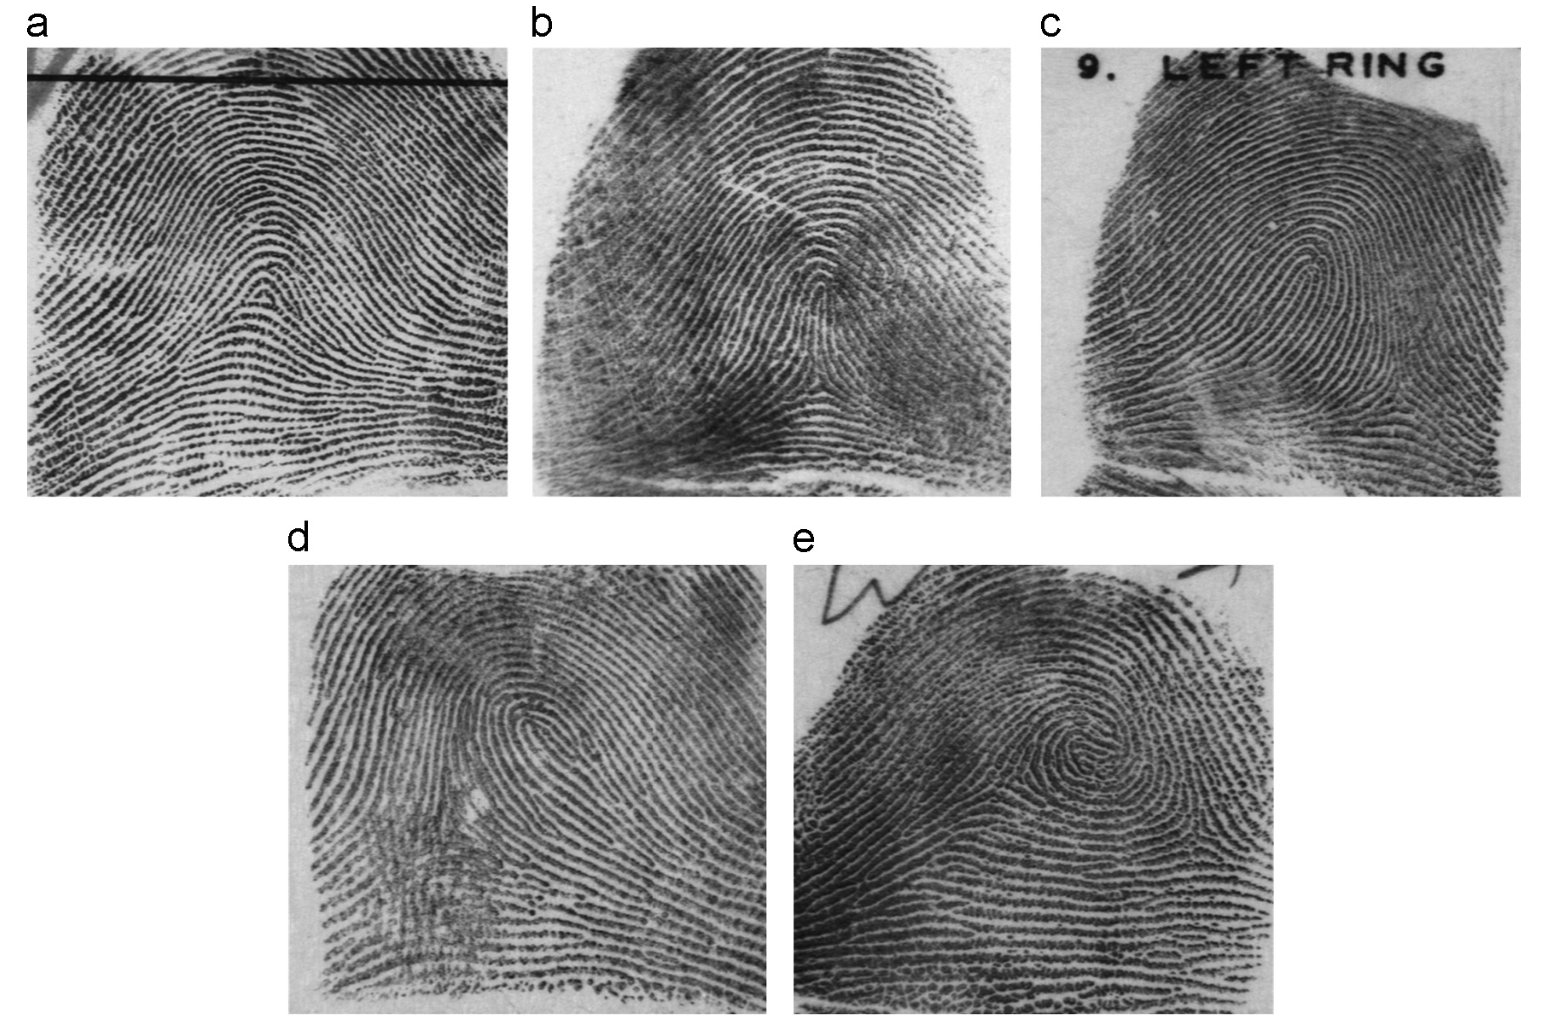
\includegraphics[width=8cm]{fig/Fingerprint_classes.png}
	\end{center}
	\caption{Examples of fingerprint classes: (a) Arch (b) Tented Arch (c) Left Loop (d) Right Loop  (e) Whorl \cite{cao2013fingerprint}} 
	\label{fig.fingerprint_classes}
\end{figure}




%-------------------------------------------------------------------------

%\section{Related Work}
%%!TEX root = main.tex

The milestone of the deep reinforcement learning is deep Q-learning(DQN)\cite{mnih2013playing}, a variant of Q-learning, proposed by DeepMind. It is the first deep learning model trying to learn control policies with reinforcement learning. In 2015, DeepMind presented an improved version of DQN\cite{mnih2015human}. Their work outperformed previous algorithms and achieved a capability comparable to that of professional human-being.
%

While DQN performs well in fully-observable environments, it achieves poor result in partially observable environments. To address this problem, Hausknecht and Stone \textit{et al.}~\cite{hausknecht2015deep} introduced the Deep Recurrent Q-Networks(DRQN). The idea is to build a recurrent neural network such as LSTM on top of the DQN model.
%

One drawback of DQN is that it needs to aggregate over time to overcome data non-stationarity. To reduce the overhead caused by experience replay, DeepMind \cite{mnih2016asynchronous} proposed a another paradigm for deep reinforcement learning: multiple agents are running in parallel asynchronously on multiple instances of the environment. Using the paradigm makes Q-learning both efficient and compatible with deep neural network at the same time. They named their best method \textit{asynchronous advantage actor-critic} (A3C). Experiments showed that A3C not only achieved better result but also required less computational cost.
%

%% Alpha go 
 More recently, AlphaGo\cite{brockman2016openai}, which is also developed by DeepMind, defeated Lee Sedol and became the first 'Artificial Intelligence' who beated 9-dan professional human Go player. Behind the AlphaGo is deep neutral network integrated with reinforcement learning improving the play strategy.


%% RDQN 
 RDQN sometimes learn unrealistically high action values because it includes a maximization step over estimated action values, which tends to
 prefer overestimated to underestimated values. This has been demonstrated in some games in the Atari 2600 domain. The idea of double Q-learning algorithm \cite{van2015deep} not only yields more accurate value estimates, but leads to much higher scores on several games. This demonstrates that the overestimations of DQN indeed lead to poorer policies and that it is beneficial to reduce them.


% liyang
% Other application of reinforcement Learning in designing game includes linear evaluation function-based learning of local shape in the game of Go \cite{silver2007reinforcement} and learning control policies for text-based games \cite{narasimhan2015language}

\section{Problem statement}

The challenge of classifying fingerprint includes: 
%
1) the quality of some fingerprints images are poor; 
%
2) the inter-class dissimilarity is small and the intra-class similarity is small; 
%
3) some fingerprints can be classified into multiple classes and there exists some ambiguity in the label.

To solve these problems, many researchers propose to use handcrafted features instead of raw fingerprint images for classification and many methods have been proposed, including ridge, orientation field, singular point.
%
Kai Cao \textit{et al.}\cite{cao2013fingerprint} propose to a novel method to extract fingerprint orientation feature and use a hierarchical classifier for classification.
%
Ruxin Wang \textit{et al.} \cite{wang2014fingerprint} also use orientation filed as feature. By adopting a stacked autoencoder , they achieve 93.1\% in four-class classification.
%

Using accurate handcrafted features can improve performance.  However, due to the existence of noise and poor image quality, the accuracy of handcrafted features cannot be guaranteed.
%
Convolutional neural network (CNN) has the capability of learning features and it can be directly applied on raw images. CNN also exhibits powerful classification capability in many areas.\cite{szegedy2016rethinking}.



%-------------------------------------------------------------------------

\section{Proposed research}
%!TEX root = main.tex

In this project, we aim to develop and implement a deep learning algorithm that takes a fingerprint image as an input and classify it into one of the five pattern class types of a) Arch; b) Tented Arch; c) Left Loop; d) Right Loop; or e) Whorl. 

\subsection{Feature Extraction}
%
We will first apply raw fingerprint images to train a CNN for classification. The outputs of some intermediate layer  of CNN will be used as features for possibly a support vector machine classifier.
%
We will consider using automated extracted features (\textit{e.g.},orientation filed) as inputs for CNN training, with the goal of combining raw images and automated features as input to train CNN.

For CNN architecture, we will first use canonical architecture ( such as 5 \textit{convolutional} + 3 \textit{fully-connected} in \textit{AlexNet}\cite{krizhevsky2012imagenet}). We will then modify the CNN architecture to improve the performance.
%
\subsection{Classifier}
%
We will consider two classifiers. The first one is the prediction layer of CNN. The values in last layer indicates the predicted probabilities of each class.
%
The second one is support vector machine (SVM whose input features comprise of the CNN’s middle or last layers.

\subsection{Data Augmentation}
%
To further improve the performance, we will use data augmentation technique to generate more training samples in order to increase the generalization ability of our model.



%-------------------------------------------------------------------------

\section{Dataset}

In this project, we will use NIST Special Database 4 \cite{nist-db-4} for our experiments. Some samples can be seen in Fig.\ref{fig.fingerprint_classes}.
%
The NIST database of fingerprint images contains 2000 8-bit gray scale fingerprint image pairs, totally 4000 images.
%
Each image is 512-by-512 pixels with 32 rows of white space at the bottom and classified using one of the five following classes: Arch, Left and Right Loops, Tented Arch, Whorl.
%
Each of the five classes has 400 pairs. Each of the fingerprint pairs are two completely different rollings of the same fingerprint.

\section{Methodology}
%!TEX root = main.tex
\subsection{A3C}
The algorithm we used to beat the baseline is the asynchronous advantage actor-critic (A3C) algorithm proposed by Volodymyr et al.~\cite{mnih2016asynchronous}. It is a policy-based model-free reinforcement learning method. This algorithm maintains a policy $\pi (a_{t}|s_{t};\theta)$ and the estimate of the value function $V(s_{t};\theta_{v})$, where $\theta$ and $\theta_{v}$ are the parameters. These two parameters are learned by taking the gradient of $\log \pi (a_{t}|s_{t};\theta) A(s_{t},a_{t};\theta,\theta_{v})$ with respect to $\theta^{\prime}$. The update of $\pi (a_{t}|s_{t};\theta)$ and $V(s_{t};\theta_{v})$ happens either after every $t_{max}$ actions or when a terminal state is reached. Combining with the idea in deep learning, we use a convolutional neural network that has one softmax output for the policy $\pi (a_{t}|s_{t};\theta)$ and one linear output for the value function $V(s_{t};\theta_{v})$.


\subsection{Policy Gradient}
The objective function:
\begin{equation*}
\begin{split}
\min_{\theta}\sum_{t=1}^N R_t (-\sum_{i=1}^{n}\textbf{I}(a_i, a_t)\log(\pi(a_i|s_t; \theta))
\end{split}
\end{equation*}
where $N$ is thte number of time step in one episode, $n$ is the number of actions
in action space, $\textbf{I}(x, y)$ is an indicator function defined as $\textbf{I}(x, y) = 1 \text{ if } x==y \text{ else } 0$.

The derive of objective function:

\begin{equation}
\begin{split}
& \max_{\theta} \textbf{E}_a(R(a)) \text{ maximize the expectation of rewards over actions} \\
& \max_{\theta} \sum_a p(a|s; \theta)R(a)
\end{split}
\end{equation}
%-------------------------------------------------------------------------

\section{Experiments}
%!TEX root = main.tex

\subsection{Dataset}

In this project, we  use NIST Special Database 4 \cite{nist-db-4} and NIST Special Database 14 \cite{nist-db-14} for our experiments. Some samples can be seen in Fig.\ref{fig.fingerprint_classes}.
%
The NIST SD4 contains $2000$ 8-bit gray scale fingerprint image pairs, totally 4000 images.
%
The size of each image is $512\times512$ and each image is classified using one of the five following classes: Arch, Left and Right Loops, Tented Arch, Whorl.
%
Each of the five classes has 400 pairs(800 images). Each of the fingerprint pairs are two completely different rollings of the same fingerprint.

%
The NIST SD14 contains $27000$ 8-bit gray scale fingerprint image pairs. There are 2700 subjects in this dataset and each subject has 10 fingerprint samples pairs. The size of each image is  $768\times832$. To fit in our network, we centrally crop $768\times768$ from the samples and resize them into $512\times512$. The distribution of fingerprint classes is as shown in Table.\ref{tab.sd14_dist}.


\begin{table}[!ht]
	\centering
	\caption{Class Distribution of NIST SD14.}
\label{tab.sd14_dist}
	\begin{tabular}{|c|c|c|c|c|}
		\hline
		\textbf{Arch} & \textbf{Left Loop} & \textbf{Right Loop} & \textbf{\begin{tabular}[c]{@{}c@{}}Tented \\ Arch\end{tabular}} & \textbf{Whorl} \\ \hline
		3.6\% & 31.9\% & 30.5\% & 3.2\% & 30.8\% \\ \hline
	\end{tabular}
\end{table}

\subsection{Experimental Setup}
We use a i7-5930K desktop with 32GB memory and a Nvidia GTX TITAN X GPU for experiments.
%
Typically, we use tensorflow 1.0.1 as the deep learning library and Adaptive Moment Estimation(Adam\cite{kingma2014adam}) as the optimization algorithm. The leaning rate is 0.0001. We also use $\ell_2$ regularization with 0.0001 weight decay rate. The batch size is 32. We run $20k$ steps and report the results.

We evaluate our approach on NIST SD4 and NIST SD14 respectively.
%
For NIST SD14 experiments, we use the samples of 80\% subjects for training, totally 2160 subjects with $43200$ images. Among these $432000$ images, 36 of them have labels that do not belong to the 5 classes. These 36 images are discarded. 
The remained data of 20\% subjects are used for testing, totally $10800$ images. 9 of these images are discarded due to the same reason above.
%

For NIST SD4 experiments,  we adopt two evaluation protocols. The first protocol is cross-sample for fair comparison with other works, where we use all the first samples(2000) in each image pair as training samples and all the second samples (2000) for testing. The second protocol is cross-finger, where we use 50\% finger samples for training and 50\% finger samples for testing. To boost the performance for NIST SD4, We use NIST SD14 data to pre-train the model.

%


In addition to 5-class fingerprint classification, we also evaluate our approach on 4-class fingerprint classification because 4 class classification are also used in other studies. 
%
To achieve 4-class classification, we merge tented arch class into arch class when training SVM.

\begin{figure*}[!ht]
	\begin{subfigure}[b]{0.25\textwidth}
		\centering
		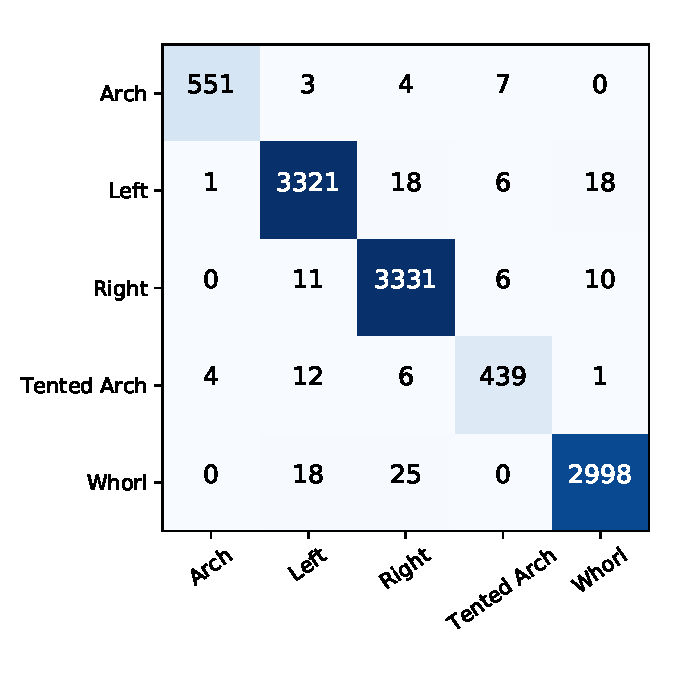
\includegraphics[width=\linewidth]{fig/figs/confusion_matrix_svm_sd14.pdf}
		\caption{SVM NIST SD14 }
		\label{fig.cnf_matrix_5class.svm_sd14}
	\end{subfigure}%
	\begin{subfigure}[b]{0.25\textwidth}
		\centering
		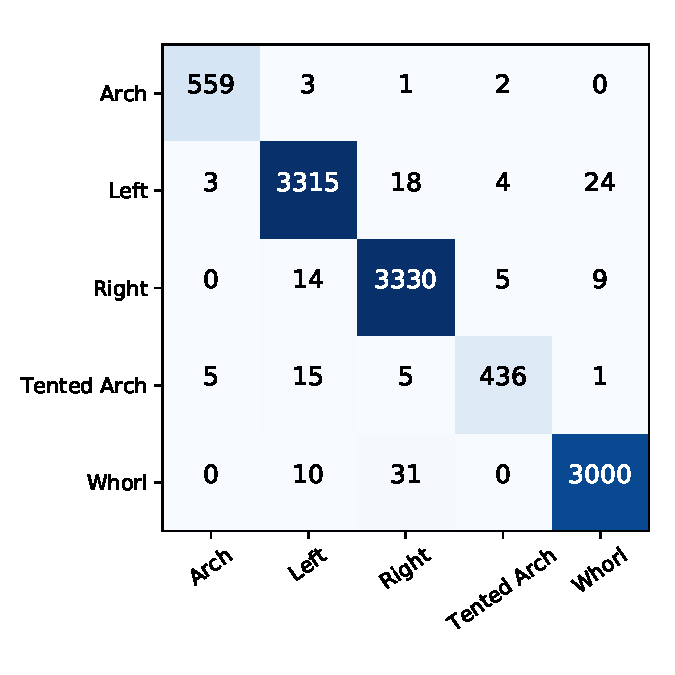
\includegraphics[width=\linewidth]{fig/figs/confusion_matrix_net_sd14.pdf}
		\caption{ConvNet NIST SD14 }
		\label{fig.cnf_matrix_5class.net_sd14}
	\end{subfigure}%
	\begin{subfigure}[b]{0.25\textwidth}
		\centering
		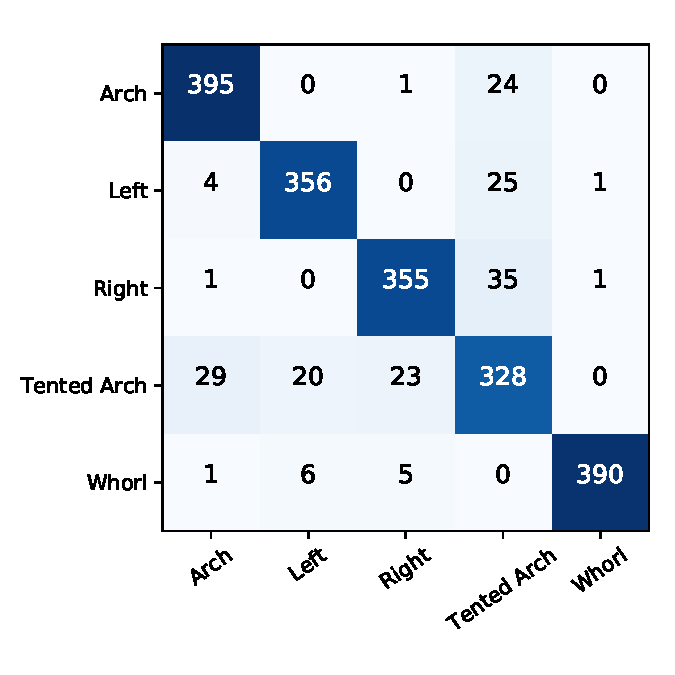
\includegraphics[width=\linewidth]{fig/figs/confusion_matrix_svm_sd4_cross_subject.pdf}
		\caption{SVM NIST SD4 }
		\label{fig.cnf_matrix_5class.svm_sd4}
	\end{subfigure}%
	\begin{subfigure}[b]{0.25\textwidth}
		\centering
		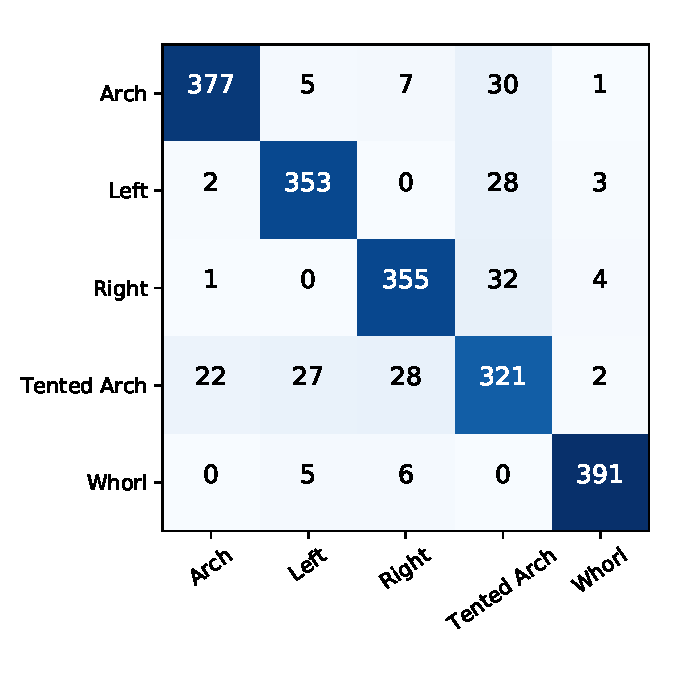
\includegraphics[width=\linewidth]{fig/figs/confusion_matrix_net_sd4_cross_subject.pdf}
		\caption{ConvNet NIST SD4 }
		\label{fig.cnf_matrix_5class.net_sd4}
	\end{subfigure}
	\caption{Confusion Matrices for 5-class classification}\label{fig.cnf_matrix_5class}
\end{figure*}

\begin{figure}[!ht]
	\begin{subfigure}[b]{0.25\textwidth}
		\centering
		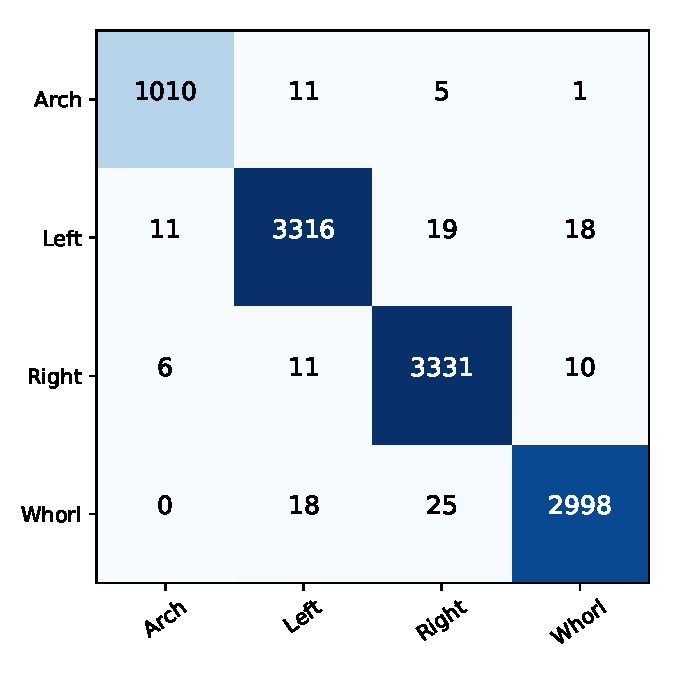
\includegraphics[width=\linewidth]{fig/figs/confusion_matrix_svm_sd14_4class.pdf}
		\caption{SVM NIST SD14 }
		\label{fig.cnf_matrix_4class.svm_sd14}
	\end{subfigure}%
	\begin{subfigure}[b]{0.25\textwidth}
		\centering
		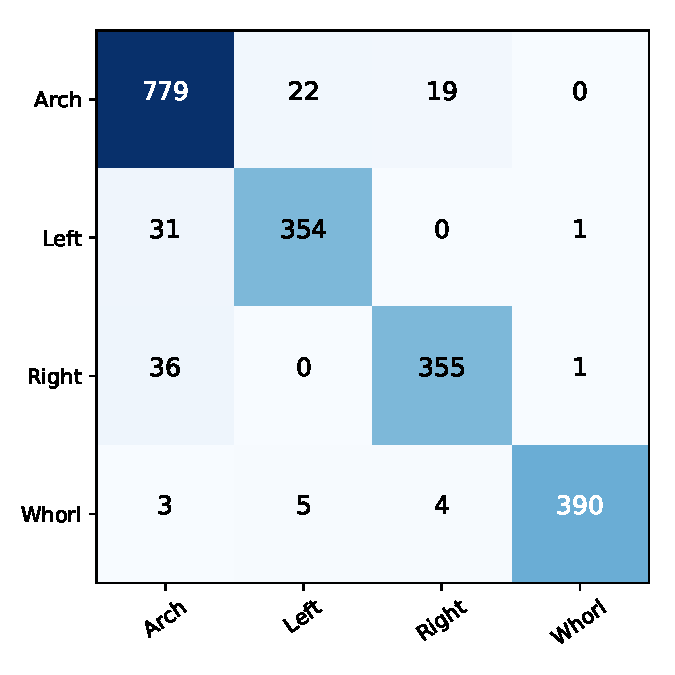
\includegraphics[width=\linewidth]{fig/figs/confusion_matrix_svm_sd4_4class_cross_subject.pdf}
		\caption{SVM NIST SD4}
		\label{fig.cnf_matrix_4class.svm_sd4}
	\end{subfigure}%

	\caption{Confusion Matrices for 4-class classification}\label{fig.cnf_matrix_4class}
\end{figure}

\subsection{NIST SD14 result}
The result for NIST SD14 is shown in Table\ref{tab.SD14_result}. In addition to report SVM performance, we also report the performance when ConvNet is used as classifier. As we can see, both ConvNet and SVM achieve the same accuracy (0.9861) for 5-class classification. However, ConvNet performs slightly better  in terms of average precision, recall rate and F1 score.
%
For 4-class classification, the 4-class SVM achieves 0.9875 accuracy.

For 5-class classification, the confusion matrix is shown in Figure.\ref{fig.cnf_matrix_5class.svm_sd14} and Figure.\ref{fig.cnf_matrix_5class.net_sd14}.
For 4-class classification, the confusion matrix is shown in Figure.\ref{fig.cnf_matrix_4class.svm_sd14}. 
%
As we can see, the number of arch and tented arch samples are relatively small compared to other classes. Our proposed approach can still achieve high accuracy despite the unbalanced distribution of fingerprint types.


\begin{table}[!ht]
	
	\centering
	\caption{ Experiment results for NIST SD14. In column 4, 5 and 6, we also report the average precision, recall and F1 score for all predicted classes. }
	\label{tab.SD14_result}
	\scalebox{0.87}{
	\begin{tabular}{|c|c|c|c|c|c|}
		\hline
		\textbf{method} & \textbf{\begin{tabular}[c]{@{}c@{}}\# of \\ classes\end{tabular}} & \textbf{accuracy} & \textbf{\begin{tabular}[c]{@{}c@{}}average \\ precision\end{tabular}} & \textbf{\begin{tabular}[c]{@{}c@{}}average\\  recall\end{tabular}} & \textbf{\begin{tabular}[c]{@{}c@{}}average \\ F1 score\end{tabular}} \\ \hline
		ConvNet & 5 & 0.9861 & 0.9843 & 0.9793 & 0.9817 \\ \hline
		SVM & 5 & 0.9861 & 0.9822 & 0.9781 & 0.9801 \\ \hline
		SVM & 4 & 0.9875 & 0.9869 & 0.9867 & 0.9868 \\ \hline
	\end{tabular}
}
\end{table}

\subsection{NIST SD4}

The result for NIST SD4 is shown in Table\ref{tab.SD4_result}. 
%
As we can see, SVM performs better than ConvNet not only in accuracy but also in average precision, recall rate and F1 score. 

The 5-class accuracy of our approach is 0.9275, which is about 0.037 lower than \cite{cao2013fingerprint}. The 4-class accuracy is 0.9495, which is about 0.022 lower than \cite{cao2013fingerprint}.
%
However, in \cite{cao2013fingerprint}, the 17\% of NIST SD4 samples they use has two labels due to ambiguity. For those samples with two labels, they use only the first label for training. When testing, the classification is considered to be correct if the output matches any one of the two labels. In our experiments, the newly downloaded NIST SD4 has only one label for each example. This is one of the reason why our performance is not as good as theirs.


For 5-class classification using cross-finger protocol, the confusion matrix is shown in Figure.\ref{fig.cnf_matrix_5class.svm_sd4} and Figure.\ref{fig.cnf_matrix_5class.net_sd4}.
For 4-class classification using cross-finger protocol, the confusion matrix is shown in Figure.\ref{fig.cnf_matrix_4class.svm_sd4}.


\begin{table}[!ht]
	\centering
	\caption{ Experiment results for NIST SD4. In column 4, 5 and 6, we also report the average precision, recall and F1 score for all predicted classes. }
	\label{tab.SD4_result}
		\scalebox{0.87}{
	\begin{tabular}{|c|c|c|c|c|c|}
		\hline
		 \textbf{method} & \textbf{\begin{tabular}[c]{@{}c@{}}\# of \\ classes\end{tabular}} & \textbf{accuracy} & \textbf{\begin{tabular}[c]{@{}c@{}}average \\ precision\end{tabular}} & \textbf{\begin{tabular}[c]{@{}c@{}}average\\  recall\end{tabular}} & \textbf{\begin{tabular}[c]{@{}c@{}}average \\ F1 score\end{tabular}} \\ \hline
		 \multicolumn{6}{|c|}{\textbf{Cross-Sample}}      \\ \hline
		ConvNet & 5 & 0.9215 & 0.9225 & 0.9215 & 0.9217 \\ \hline
		SVM & 5 & 0.9275 & 0.9325 & 0.9275 & 0.9288 \\ \hline
		SVM & 4 & 0.9495 & 0.9576 & 0.9459 & 0.9514 \\ 
\hhline{|======|}
\multicolumn{6}{|c|}{\textbf{Cross-Finger}}      \\ \hline
		ConvNet & 5 & 0.8985 & 0.8991 & 0.8986 & 0.8987 \\ \hline
SVM & 5 & 0.9120 & 0.9132 & 0.9117 & 0.9123 \\ \hline
SVM & 4 & 0.9390 & 0.9452 & 0.9357 & 0.9403 \\ \hline
		
\end{tabular}}
\end{table}


\begin{table}[!ht]
	\centering
	\caption{Experiment results for NIST SD4 with two labels.}
	\label{tab.SD4_result_two_labels}
	\begin{tabular}{|c|c|c|c|}
		\hline
		\textbf{method} & \textbf{\# of classes} & \textbf{accuracy} & \textbf{protocol} \\ \hline
		ConvNet & 5 & 0.9535 & cross-sample \\ \hline
		SVM & 5 & 1.0 & cross-sample \\ \hline
		SVM & 4 & 1.0 & cross-sample \\ \hline
		\cite{cao2013fingerprint} & 5 & 0.959 & cross-sample \\ \hline
		\cite{cao2013fingerprint}& 4 & 0.972 & cross-sample \\ \hline
		\cite{wang2014fingerprint} & 4 & 0.980 & not-spepcified \\ \hline
		ConvNet & 5 & 0.945 & cross-finger \\ \hline
		SVM & 5 & 1.0 & cross-finger \\ \hline
		SVM & 4 & 1.0 & cross-finger \\ \hline
	\end{tabular}
\end{table}



%-------------------------------------------------------------------------


\section{Conclusion}
%!TEX root = main.tex

In this paper, we propose a deep learning approach for automatic fingerprint type classification. We design a deep ConvNet based on residual network. To preserve as much fingerprint details as possible, the input image is designed to be  $512\times512$ and we can use two early convolutional layers to reduce the computational cost. The deep ConvNet serves as a feature extractor and on top of that a SVM is trained as the final classifier. Experiment results show that the proposed automatic that does not rely on any hand-crafted features can achieve high accuracy comparable to the state-of-the-art approach even if only label is used. Our proposed can accurately predict the fingerprint class using raw images, avoiding the need of using orientation filed estimation. Future works include using more advanced deep networks and ensemble techniques to fuse multiple classifiers.

{\small
\bibliographystyle{ieee}
\bibliography{egbib}
}

\end{document}
